\subsection{Singular Value Decomposition (SVD) ($A = U \Sigma V^\top$)}



\begin{enumerate}
    \item The singular value decomposition (SVD) of a matrix is a central matrix decomposition method in linear algebra.
    \hfill \cite{mfml/book/mml/Deisenroth-Faisal-Ong}

    \item It has been referred to as the “fundamental theorem of linear algebra” because it can be applied to \textbf{all matrices}, not only to square matrices, and it \textbf{always exists}.
    \hfill \cite{mfml/book/mml/Deisenroth-Faisal-Ong}

    \item the SVD of a matrix $\bm{A}$, which represents a linear mapping $\Phi : V \to W$, quantifies the change between the underlying geometry of these two vector spaces.
    \hfill \cite{mfml/book/mml/Deisenroth-Faisal-Ong}

    \item
    \begin{theorem}[SVD Theorem]
        Let $\bm{A} \in \mbbR^{m\times n}$ be a rectangular matrix of rank $r \in [0,\ \min(m, n)]$.
        The SVD of $\bm{A}$ is a decomposition of the form
        $
            \underset{\displaystyle m\times n}{\bm{A}} =
            \underset{\displaystyle m\times m}{\bm{U}}\
            \underset{\displaystyle m\times n}{\bm{\Sigma}}\
            \underset{\displaystyle n\times n}{\bm{V}^\top}
        $
        with an orthogonal matrix $\bm{U} \in \mbbR^{m\times m}$ with column vectors $\bm{u}_i$ , $i = 1, \cdots , m$, and an orthogonal matrix $\bm{V} \in \mbbR^{n\times n}$ with column vectors $\bm{v}_j$ , $j = 1, \cdots , n$.
        Moreover, $\bm{\Sigma}$ is an $m \times n$ matrix with $\Sigma_{ii} = \sigma_i \geq 0$ and $\Sigma_{ij} = 0, i \neq j$.
        \hfill \cite{mfml/book/mml/Deisenroth-Faisal-Ong}
    \end{theorem}

    \item $\bm{U}$
    \begin{enumerate}
        \item $\bm{u}_i$ are called the left-singular vectors
        \hfill \cite{mfml/book/mml/Deisenroth-Faisal-Ong}
    \end{enumerate}

    \item $\bm{\Sigma}$:
    \begin{enumerate}
        \item The diagonal entries $\sigma _i$ , $i = 1, \cdots , r$, of $\bm{\Sigma}$  are called the singular values
        \hfill \cite{mfml/book/mml/Deisenroth-Faisal-Ong}

        \item By convention, the singular values are ordered, i.e., $\sigma _1 \geq \sigma _2 \geq \sigma _r \geq 0$.
        \hfill \cite{mfml/book/mml/Deisenroth-Faisal-Ong}

        \item The singular value matrix $\bm{\Sigma}$ is unique
        \hfill \cite{mfml/book/mml/Deisenroth-Faisal-Ong}

        \item the $\bm{\Sigma}$ is rectangular, particularly, it is of the same size as $\bm{A}$
        \hfill \cite{mfml/book/mml/Deisenroth-Faisal-Ong}

        \item $\bm{\Sigma}$ has a diagonal submatrix that contains the singular values and needs additional zero padding
        \hfill \cite{mfml/book/mml/Deisenroth-Faisal-Ong}
        \\
        if $m > n$, then the matrix $\bm{\Sigma}$ has diagonal structure up to row $n$ and then consists of $\bm{0}^\top$ row vectors from $n + 1$ to $m$ below so that:
        \hfill \cite{mfml/book/mml/Deisenroth-Faisal-Ong}
        \\
        .\hfill
        $
            \begin{bmatrix}
                \sigma_1 & \cdots  & 0 \\
                \vdots & \ddots & \vdots \\
                0 & \cdots & \sigma_n \\
                0 & \cdots & 0\\
                0 & \ddots & 0 \\
                0 & \cdots & 0\\
            \end{bmatrix}
        $
        \hfill \cite{mfml/book/mml/Deisenroth-Faisal-Ong}
        \\
        If $m < n$, the matrix $\bm{\Sigma}$ has a diagonal structure up to column $m$ and columns that consist of $\bm{0}$ from $m + 1$ to $n$:
        \hfill \cite{mfml/book/mml/Deisenroth-Faisal-Ong}
        \\
        .\hfill
        $
            \begin{bmatrix}
                \sigma_1 & \cdots  & 0 & 0 & 0 & 0 \\
                \vdots & \ddots & \vdots & \vdots  & \ddots & \vdots \\
                0 & \cdots & \sigma_m & 0 & 0 & 0 \\
            \end{bmatrix}
        $
        \hfill \cite{mfml/book/mml/Deisenroth-Faisal-Ong}
    \end{enumerate}



    \item $\bm{V}$
    \begin{enumerate}
        \item $\bm{v}_j$ are called the right-singular vectors
        \hfill \cite{mfml/book/mml/Deisenroth-Faisal-Ong}

    \end{enumerate}


    \item \begin{definition}[Standard SVD/ Full SVD ($A = U\Sigma V^\top$)]
        SVD notation where the SVD is described as having two square left- and right-singular vector matrices, but a non-square singular value matrix.
        \hfill \cite{mfml/book/mml/Deisenroth-Faisal-Ong}
        \\
        $
            \underset{\displaystyle m\times n}{\bm{A}} =
            \underset{\displaystyle m\times m}{\bm{U}}\
            \underset{\displaystyle m\times n}{\bm{\Sigma}}\
            \underset{\displaystyle n\times n}{\bm{V}^\top}
        $
        \hfill \cite{mfml/book/mml/Deisenroth-Faisal-Ong}
    \end{definition}

    \item \begin{definition}[Reduced SVD ($A = U_r\Sigma_r V_r^\top$)]
         focus on square singular matrices
         \hfill \cite{mfml/book/mml/Deisenroth-Faisal-Ong}
         \\
         $
            \underset{\displaystyle m\times n}{\bm{A}} =
            \underset{\displaystyle m\times n}{\bm{U}_r}\
            \underset{\displaystyle n\times n}{\bm{\Sigma}_r}\
            \underset{\displaystyle n\times n}{\bm{V}_r^\top}
        $
        \hfill ($m \geq n$)
        \hfill \cite{mfml/book/mml/Deisenroth-Faisal-Ong}
        \\
        This alternative format changes merely how the matrices are constructed but leaves the mathematical structure of the SVD unchanged.
        The convenience of this alternative formulation is that $\bm{\Sigma}$ is diagonal, as in the eigenvalue decomposition.
        \hfill \cite{mfml/book/mml/Deisenroth-Faisal-Ong}
    \end{definition}

    \item
    \begin{definition}[Compact SVD/ Thin SVD/ Truncated SVD ($A = U\Sigma V$)]
        It is possible to define the SVD of a rank-$r$ matrix $\bm{A}$ so that $\bm{U}$ is an $m \times r$ matrix, $\bm{\Sigma}$ a diagonal matrix $r \times r$, and $\bm{V}$ an $r \times n$ matrix.
        This construction is very similar to our definition, and ensures that the diagonal matrix $\bm{\Sigma}$ has only nonzero entries along the diagonal.
        The main convenience of this alternative notation is that $\bm{\Sigma}$ is diagonal, as in the eigenvalue decomposition.
        \\
         $
            \underset{\displaystyle m\times n}{\bm{A}} =
            \underset{\displaystyle m\times r}{\bm{U}}\
            \underset{\displaystyle r\times r}{\bm{\Sigma}}\
            \underset{\displaystyle r\times n}{\bm{V}}
        $
        \hfill \cite{mfml/book/mml/Deisenroth-Faisal-Ong}
    \end{definition}

    \item A restriction that the SVD for $\bm{A}$ only applies to $m \times n$ matrices with $m > n$ is practically unnecessary.
    When $m < n$, the SVD decomposition will yield $\bm{\Sigma}$ with more zero columns than rows and, consequently, the singular values $\sigma _{m+1}, \cdots , \sigma _n$ are $0$.
    \hfill \cite{mfml/book/mml/Deisenroth-Faisal-Ong}
\end{enumerate}





\subsubsection{Geometric Intuitions for the SVD}

\begin{figure}[H]
    \centering
    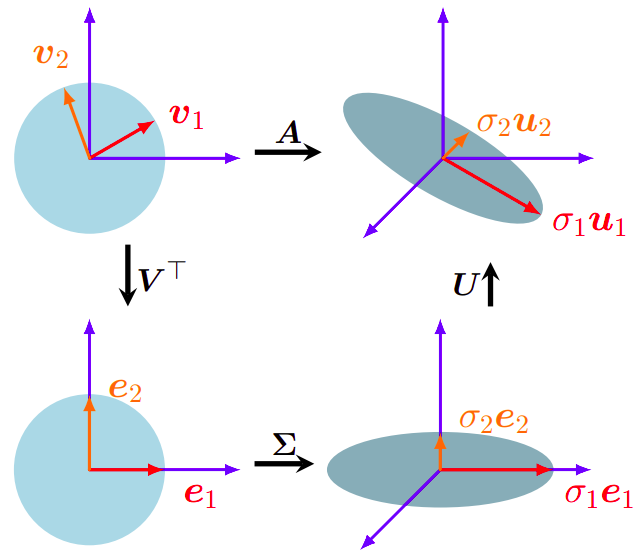
\includegraphics[
        width=\linewidth,
        height=5cm,
        keepaspectratio,
    ]{images/maths-for-ml/singular-value-decomposition.png}
    \caption*{
        Intuition behind the SVD of a matrix $\bm{A} \in \mbbR^{3\times 2}$ as sequential transformations.
        \hfill \cite{mfml/book/mml/Deisenroth-Faisal-Ong}
        \\
        \textbf{Top-left to bottom-left}: $\bm{V}^\top$ performs a basis change in $\mbbR^2$.
        \hfill \cite{mfml/book/mml/Deisenroth-Faisal-Ong}
        \\
        \textbf{Bottom-left to bottom-right}: $\Sigma$ scales and maps from $\mbbR^2$ to $\mbbR^3$ . The ellipse in the bottom-right lives in $\mbbR^3$. The third dimension is orthogonal to the surface of the elliptical disk.
        \hfill \cite{mfml/book/mml/Deisenroth-Faisal-Ong}
        \\
        \textbf{Bottom-right to top-right}: $\bm{U}$ performs a basis change within $\mbbR^3$.
        \hfill \cite{mfml/book/mml/Deisenroth-Faisal-Ong}
    }
\end{figure}

SVD as sequential linear transformations performed on the bases.
The SVD of a matrix can be interpreted as a decomposition of a corresponding linear mapping $\Phi : \mbbR^n \to \mbbR^m$ into three operations.
Assume we are given a transformation matrix of a linear mapping $\Phi : \mbbR^n \to \mbbR^m$ with respect to the standard bases $B$ and $C$ of $\mbbR^n$ and $\mbbR^m$, respectively.
Moreover, assume a second basis $\tilde{B}$ of $\mbbR^n$ and $\tilde{C}$ of $\mbbR^m$. Then:
\hfill \cite{mfml/book/mml/Deisenroth-Faisal-Ong}

\begin{enumerate}
    \item The matrix $\bm{V}$ performs a basis change in the domain $\mbbR^n$ from $\tilde{B}$ (represented by the red and orange vectors $\bm{v}_1$ and $\bm{v}_2$ in the top-left) to the standard basis $B$.
    $\bm{V}^\top = \bm{V}^{-1}$ performs a basis change from $B$ to $\tilde{B}$.
    The red and orange vectors are now aligned with the canonical basis in the bottom-left.
    \hfill \cite{mfml/book/mml/Deisenroth-Faisal-Ong}

    \item Having changed the coordinate system to $\tilde{B}$, $\bm{\Sigma}$ scales the new coordinates by the singular values $\sigma _i$ (and adds or deletes dimensions), i.e., $\bm{\Sigma}$  is the transformation matrix of $\Phi$ with respect to $\tilde{B}$ and $\tilde{C}$, represented by the red and orange vectors being stretched and lying in the $\bm{e}_1-\bm{e}_2$ plane, which is now embedded in a third dimension in the bottom-right.
    \hfill \cite{mfml/book/mml/Deisenroth-Faisal-Ong}

    \item $\bm{U}$ performs a basis change in the co-domain $\mbbR^m$ from $\tilde{C}$ into the canonical basis of $\mbbR^m$, represented by a rotation of the red and orange vectors out of the $\bm{e}_1-\bm{e}_2$ plane.
    This is shown in the top-right.
    \hfill \cite{mfml/book/mml/Deisenroth-Faisal-Ong}

    \item The SVD expresses a change of basis in both the domain and codomain.
    What makes the SVD special is that these two different bases are simultaneously linked by the singular value matrix $\bm{\Sigma}$.
    \hfill \cite{mfml/book/mml/Deisenroth-Faisal-Ong}
\end{enumerate}



\subsubsection{Construction of the SVD}

\begin{enumerate}
    \item Finding $\bm{V}$:
    \begin{enumerate}
        \item $
            \bm{A}^\top \bm{A}
            = \bm{PDP} ^\top
            = \bm{P} \begin{bmatrix}
                \lambda_1 & \cdots & 0 \\
                \vdots & \ddots & \vdots \\
                0 & \cdots & \lambda_n
            \end{bmatrix} \bm{P} ^\top
            \in \mbbR^{n\times n}
        $
        \hfill \cite{mfml/book/mml/Deisenroth-Faisal-Ong}

        \item $\bm{P}$ is an orthogonal matrix, which is composed of the orthonormal eigenbasis.
        \hfill \cite{mfml/book/mml/Deisenroth-Faisal-Ong}

        \item The $\lambda_i \geq 0$ are the eigenvalues of $\bm{A}^\top \bm{A}$.
        \hfill \cite{mfml/book/mml/Deisenroth-Faisal-Ong}

        \item Let SVD exist. Then:
        \hfill \cite{mfml/book/mml/Deisenroth-Faisal-Ong}
        \\
        $
            \bm{A}^\top \bm{A}
            = (\bm{U\Sigma V}^\top)^\top (\bm{U\Sigma V}^\top)
            = \bm{V} \bm{\Sigma}^\top \bm{U}^\top \bm{U\Sigma V}^\top
            = \bm{V} \bm{\Sigma}^\top \bm{\Sigma V}^\top
            = \bm{V} \begin{bmatrix}
                \sigma_1^2 & \cdots & 0 \\
                \vdots & \ddots & \vdots \\
                0 & \cdots & \sigma_n^2
            \end{bmatrix} \bm{V} ^\top
            \in \mbbR^{n\times n}
        $
        \hfill \cite{mfml/book/mml/Deisenroth-Faisal-Ong}

        \item $\bm{V}^\top = \bm{P}^\top$ and $\sigma^2_i = \lambda_i$
        \hfill \cite{mfml/book/mml/Deisenroth-Faisal-Ong}

        \item Therefore, the eigenvectors of $\bm{A}^\top \bm{A}$ that compose $\bm{P}$ are the right-singular vectors $\bm{V}$ of $\bm{A}$
        \hfill \cite{mfml/book/mml/Deisenroth-Faisal-Ong}

        \item The eigenvalues of $\bm{A}^\top \bm{A}$ are the squared singular values of $\bm{\Sigma}$
        \hfill \cite{mfml/book/mml/Deisenroth-Faisal-Ong}
    \end{enumerate}

    \item Finding $\bm{U}$:
    \begin{enumerate}
        \item $
            \bm{A}^\top \bm{A}
            = \bm{SDS} ^\top
            = \bm{S} \begin{bmatrix}
                \lambda_1 & \cdots & 0 \\
                \vdots & \ddots & \vdots \\
                0 & \cdots & \lambda_m
            \end{bmatrix} \bm{S} ^\top
            \in \mbbR^{m\times m}
        $
        \hfill \cite{mfml/book/mml/Deisenroth-Faisal-Ong}

        \item $\bm{P}$ is an orthogonal matrix, which is composed of the orthonormal eigenbasis.
        \hfill \cite{mfml/book/mml/Deisenroth-Faisal-Ong}

        \item Let SVD exist. Then:
        \hfill \cite{mfml/book/mml/Deisenroth-Faisal-Ong}
        \\
        $
            \bm{A} \bm{A} ^\top
            = (\bm{U\Sigma V}^\top) (\bm{U\Sigma V}^\top) ^\top
            = \bm{U\Sigma V}^\top \bm{V} \bm{\Sigma}^\top \bm{U}^\top
            = \bm{U} \bm{\Sigma} \bm{\Sigma}^\top \bm{U}^\top
            = \bm{U} \begin{bmatrix}
                \sigma_1^2 & \cdots & 0 \\
                \vdots & \ddots & \vdots \\
                0 & \cdots & \sigma_m^2
            \end{bmatrix} \bm{U} ^\top
            \in \mbbR^{m\times m}
        $
        \hfill \cite{mfml/book/mml/Deisenroth-Faisal-Ong}

        \item $\bm{U}^\top = \bm{S}^\top$ and $\sigma^2_i = \lambda_i$
        \hfill \cite{mfml/book/mml/Deisenroth-Faisal-Ong}

        \item The orthonormal eigenvectors of $\bm{AA}^\top$ are the left-singular vectors $\bm{U}$ and form an orthonormal basis in the codomain of the SVD.
        \hfill \cite{mfml/book/mml/Deisenroth-Faisal-Ong}
    \end{enumerate}

    \item Finding $\bm{\Sigma}$:
    \begin{enumerate}
        \item Since $\bm{AA^\top}$ and $\bm{A ^\top A}$ have the same nonzero eigenvalues, the nonzero entries of the $\bm{\Sigma}$ matrices in the SVD for both cases have to be the same.
        \hfill \cite{mfml/book/mml/Deisenroth-Faisal-Ong}

        \item  the images of the $\bm{v}_i$ under $\bm{A}$ have to be orthogonal, too.
        \hfill \cite{mfml/book/mml/Deisenroth-Faisal-Ong}
        \\
        $
            (\bm{Av}_i)^\top (\bm{Av}_j ) =
            \bm{v}^\top _i(\bm{A}^\top \bm{A})\bm{v}_j =
            \bm{v}^\top _i(\lambda _j\bm{v}_j ) =
            \lambda _j\bm{v}^\top _i \bm{v}_j
            = 0
        $
        \hfill \cite{mfml/book/mml/Deisenroth-Faisal-Ong}

        \item For the case $m \geq r$ (where $r = rk(\bm{A})$), it holds that $\dCurlyBrac{\bm{Av}_1, \cdots , \bm{Av}_r}$ is a basis of an r-dimensional subspace of $\mbbR^m$.
        \hfill \cite{mfml/book/mml/Deisenroth-Faisal-Ong}

        \item To complete the SVD construction, we need left-singular vectors that are orthonormal:
        We normalize the images of the right-singular vectors $\bm{Av}_i$ and obtain:
        \hfill \cite{mfml/book/mml/Deisenroth-Faisal-Ong}
        \\
        $
            \bm{u}_i = \dfrac{\bm{Av}_i}{\dnorm{\bm{Av}_i}}
            = \dfrac{\bm{Av}_i}{\sqrt{\lambda_i}}
            = \dfrac{\bm{Av}_i}{\sigma_i}
            \hspace{0.3cm}
            \Rightarrow
            \bm{Av}_i = \sigma_i \bm{u}_i
        $
        \hfill
        $
            (i = 1, \cdots , r)
        $
        \hfill \cite{mfml/book/mml/Deisenroth-Faisal-Ong}

        \item singular value equation: $\bm{Av}_i = \sigma_i \bm{u}_i$
        \hfill \cite{mfml/book/mml/Deisenroth-Faisal-Ong}

        \item \textbf{Author's Note}: As $\bm{V}^T = \bm{V}^{-1}$,
        \\
        $
            \bm{A} = \bm{U\Sigma V}^\top = \bm{U\Sigma V}^{-1}
            \hspace{0.5cm}
            \Rightarrow
            \bm{AV} = \bm{U\Sigma}
            \hspace{0.5cm}
            \Rightarrow
            \bm{U} = \bm{AV\Sigma}^{-1}
            \hspace{0.5cm}
            \Rightarrow
            \bm{U} = \dfrac{\bm{AV}}{\bm{\Sigma}}
        $
        \\
        As $\bm{\Sigma}$ is a diagonal matrix (more or less), $\bm{\Sigma}^{-1} = \dfrac{1}{\bm{\Sigma}}$ (element-wise)

    \end{enumerate}

    \item the eigenvectors of $\bm{A} ^\top \bm{A}$, which we know are the right-singular vectors $\bm{v}_i$ , and their normalized images under $\bm{A}$, the left-singular vectors $\bm{u}_i$ , form two self-consistent ONBs that are connected through the singular value matrix $\bm{\Sigma}$.
    \hfill \cite{mfml/book/mml/Deisenroth-Faisal-Ong}

    \item Case 1: $n<m$:
    \begin{enumerate}
        \item $\bm{Av}_i = \sigma_i \bm{u}_i$ holds for $i\leq n$, i.e., only for the nonzero singular values.
        \hfill \cite{mfml/book/mml/Deisenroth-Faisal-Ong, common/online/chatgpt}

        \item For $i>n$, $\bm{u} _i$  are not defined via $\bm{Av}_ i$ .
        \hfill \cite{mfml/book/mml/Deisenroth-Faisal-Ong, common/online/chatgpt}

        \item But by construction of SVD, we choose $\bm{u}_ i$  to complete an orthonormal basis for $\mbbR^ m$ , so the extra $\bm{u}_ i$ 's (for $i>n$) are orthonormal anyway.
        \hfill \cite{mfml/book/mml/Deisenroth-Faisal-Ong, common/online/chatgpt}
    \end{enumerate}

    \item Case 2: $m<n$
    \begin{enumerate}
        \item $\bm{Av}_i = \sigma_i \bm{u}_i$ only holds for $i\leq m$.
        \hfill \cite{mfml/book/mml/Deisenroth-Faisal-Ong, common/online/chatgpt}

        \item For $i>m$, $\bm{Av}_ i =0$. So, these $\bm{v}_ i$  lie in the null space of $\bm{A}$.
        \hfill \cite{mfml/book/mml/Deisenroth-Faisal-Ong, common/online/chatgpt}

        \item The set of all $\bm{v}_ i$  (even for $i>m$) is still orthonormal.
        \hfill \cite{mfml/book/mml/Deisenroth-Faisal-Ong, common/online/chatgpt}

        \item So the columns $\bm{v}_ i$  with $i>m$ form an orthonormal basis for the null space of $\bm{A}$.
        \hfill \cite{mfml/book/mml/Deisenroth-Faisal-Ong, common/online/chatgpt}
    \end{enumerate}
\end{enumerate}





